\documentclass[sigconf,nonacm]{acmart}

\settopmatter{printacmref=false,printfolios=true}
\setcopyright{none}
\renewcommand\footnotetextcopyrightpermission[1]{}

\usepackage{amsmath}
\usepackage{tabularx}
\usepackage{array}
\usepackage{enumitem}
\usepackage{balance}
\usepackage{float}
\usepackage{xurl}

\definecolor{CourseBlue}{HTML}{315EFB}
\definecolor{CourseTeal}{HTML}{14877D}

\hypersetup{
    colorlinks=true,
    linkcolor=CourseBlue,
    citecolor=CourseTeal,
    urlcolor=CourseTeal
}

\newcolumntype{Y}{>{\raggedright\arraybackslash}X}

\setlist{
    leftmargin=*,
    topsep=3pt,
    itemsep=2pt
}

% ------------------------------------------------------------
% Paragraph formatting
% ------------------------------------------------------------

\setlength{\parindent}{0pt}
\setlength{\parskip}{0pt}

% ------------------------------------------------------------
% Course metadata
% ------------------------------------------------------------

\newcommand{\CourseNumber}{COMSCI/ECON 206}
\newcommand{\CourseName}{Computational Microeconomics}
\newcommand{\CourseSession}{Autumn 2026 Session 1}
\newcommand{\Instructor}{Luyao Zhang}
\newcommand{\WorkshopSession}{Trust and Deception}

\newcommand{\GitHubLink}{
\url{https://github.com/GihoonE/cs206-overleaf-template}
}

\newcommand{\ColabLink}{
\url{https://colab.research.google.com/drive/1X3pShVdZfKDuHvvDRv116KbVT8oVtQv0?usp=sharing}
}

\newcommand{\DemoLink}{
\url{https://huggingface.co/spaces/dku-comsci-econ206-2026/gihun-space}
}

\newcommand{\coursemeta}{
\noindent
\textbf{Submission to:}
\CourseNumber{} --- \CourseName.\\
\textbf{Course session:}
\CourseSession.
\textbf{Workshop:}
\WorkshopSession.\\
\textbf{Instructor:}
\Instructor.
\textbf{Assignment:}
PS1 research proposal.

\vspace{0.5em}
}

% ------------------------------------------------------------
% Title
% ------------------------------------------------------------

\title{
Toward a Standardized Unit of AI Usage:
Making Heterogeneous LLM and Agent Services Comparable
}

\author{Gihun Lee}

\affiliation{
    \institution{Duke Kunshan University}
    \city{Kunshan}
    \country{China}
}

\email{gihun.lee@dukekunshan.edu.cn}

\renewcommand{\shortauthors}{Lee}


\begin{document}

% ============================================================
% FIGURE 1
% ============================================================

\begin{teaserfigure}

\captionsetup{skip=8pt}
\centering

% Use the PNG if it exists.
% If it is missing, the document will still compile.
\IfFileExists{figures/ps1_teaser.png}{
    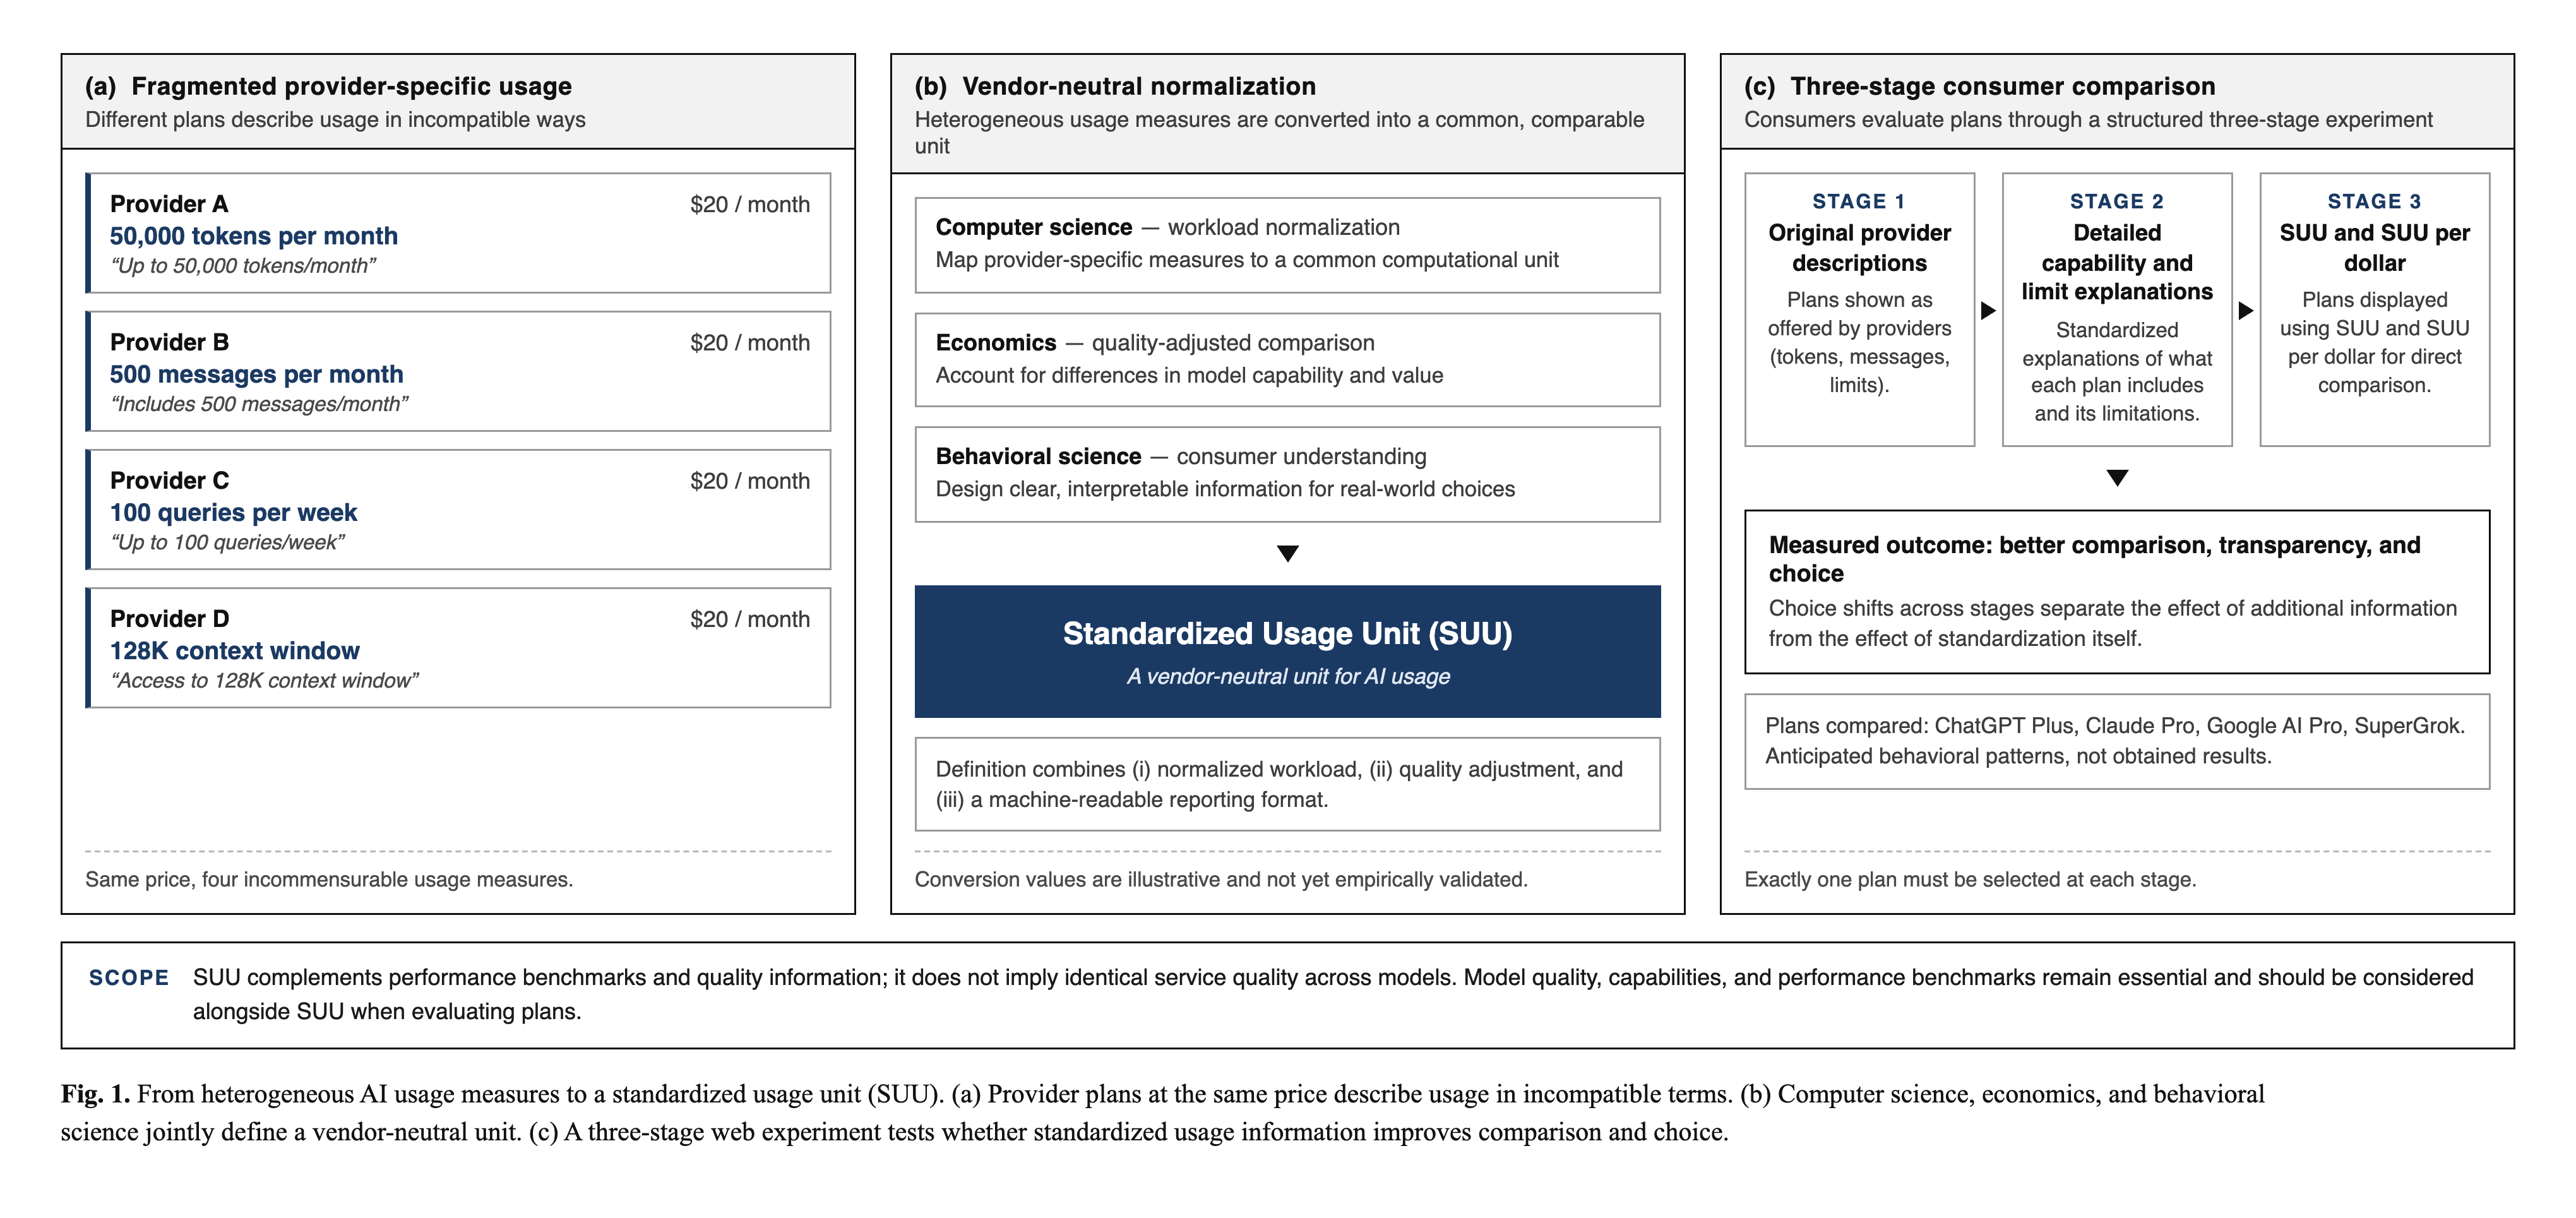
\includegraphics[
        width=\textwidth
    ]{figures/ps1_teaser.png}
}{
    \fbox{
        \parbox[c][3.0cm][c]{0.94\textwidth}{
            \centering
            Figure 1 placeholder:
            SUU computational and behavioral framework
        }
    }
}

\caption{
Proposed Standardized Usage Unit (SUU) framework.
Provider-specific prices and usage constraints are converted into
workload-specific service capacities for reasoning, coding, and agentic tasks.
These capacities are adjusted using normalized benchmark performance to produce
Reasoning SUU, Coding SUU, and Agentic SUU; Overall SUU is their equal-weight
average. The three-stage behavioral design compares decisions made with
(1) original provider information,
(2) expanded capability and limit information,
and (3) SUU and SUU-per-dollar information.
}

\Description{
A diagram showing four AI subscription providers feeding provider-specific
prices and usage limits into a normalization pipeline. The pipeline produces
reasoning, coding, and agentic standardized usage units and their equal-weight
overall score. A three-stage experiment compares consumer choices before and
after standardized information is introduced.
}

\label{fig:teaser}

\end{teaserfigure}


\maketitle
\raggedbottom
\coursemeta


% ============================================================
% 1. THREE CONNECTED RESEARCH QUESTIONS
% ============================================================

\section{Three connected research questions}

AI subscription services expose increasingly heterogeneous LLMs and agents, yet
describe usage through provider-specific tokens, messages, rolling windows,
weekly pools, and feature-dependent limits. Model capability can already be
compared through common benchmarks, as illustrated by the Tencent benchmark
dashboard I observed, but the quantity of usable service remains difficult to
compare across providers. This project proposes a vendor-neutral
\emph{Standardized Usage Unit} (SUU) that complements performance information
rather than replacing it.

\vspace{0.5em}

\textbf{Q1---Economics:}
How does standardized, quality-aware usage information change the comparison
and perceived value of competing AI subscription plans?

\vspace{0.35em}

\textbf{Q2---Computation:}
How can heterogeneous provider limits and model capabilities be converted
reproducibly into comparable reasoning, coding, and agentic usage units?

\vspace{0.35em}

\textbf{Q3---Behavior:}
Does SUU improve consumers' understanding and plan selection, or can
standardization itself create anchoring and false comparability?

\vspace{0.5em}

Figure~\ref{fig:teaser} connects the three questions:
computation constructs comparability,
economics interprets value,
and behavioral science tests whether the standardized information improves
decision making.


% ============================================================
% 2. ECONOMICS
% ============================================================

\section{Answer to Q1: incentives and intellectual lineage}

Consider consumer $i$ choosing plan $p\in\mathcal{P}$.
Let $P_p$ denote monthly price and let

\[
\mathbf{A}_p
=
(A_{p,R},A_{p,C},A_{p,A})
\]

denote usable reasoning, coding, and agentic service.
A benchmark consumer decision is

\[
p_i^*
=
\arg\max_{p\in\mathcal P}
\left[
V_i(\mathbf{A}_p,\mathbf{Q}_p;\theta_i)
-
P_p
\right],
\]

where $\mathbf{Q}_p$ represents model capability and
$\theta_i$ captures consumer $i$'s workload needs.

\vspace{0.5em}

The consumer is the player, the action is the choice of subscription plan,
and the payoff is the perceived value of usable, quality-adjusted AI service
minus its price. The decision occurs after the provider presents price,
capability, and usage information. Consumers observe the disclosed information
but may not know how provider-specific usage units translate across competing
services.

\vspace{0.5em}

Following quality-adjusted price comparison~\cite{ehrlich2026},
my provisional hypothesis is that standardized usage information reduces
comparison costs and helps consumers select plans that better match their
workloads.

The experimental information structure changes sequentially:
Stage 1 shows original provider descriptions,
Stage 2 clarifies capabilities and limits,
and Stage 3 adds SUU.

For the current one-consumer benchmark, the decision rule is
utility-maximizing plan choice under the disclosed information.
For the later strategic disclosure extension, Bayesian equilibrium is
the solution concept under incomplete information~\cite{harsanyi1968}.

A later strategic extension could allow providers to choose how much usage
information to disclose and study how consumer beliefs respond to that disclosure.


% ============================================================
% 3. COMPUTATION
% ============================================================

\section{Answer to Q2: method and evaluation}

For provider $p$ and workload
$j\in\{R,C,A\}$---reasoning, coding, and agentic---let
$C_{p,j}$ denote the number of standardized reference tasks supported by the
plan's binding usage constraints.

Let $K_j$ denote the set of benchmark tasks associated with workload
$j\in\{R,C,A\}$, and let $S_{p,k}$ be provider $p$'s score on benchmark $k$.

\vspace{0.4em}

Each benchmark is normalized against the best-performing compared provider,
and the normalized scores are averaged within each workload:

\[
B_{p,j}
=
\frac{1}{|K_j|}
\sum_{k\in K_j}
\frac{S_{p,k}}
{\max_q S_{q,k}}.
\]

For readability, all reported benchmark-quality scores below are
shown on a 0--100 scale, i.e., as $100B_{p,j}$; the SUU definition
uses the corresponding 0--1 value $B_{p,j}$.

The workload-specific Standardized Usage Unit is

\[
\boxed{
\mathrm{SUU}_{p,j}
=
C_{p,j}B_{p,j}
}.
\]

Overall SUU is the equal-weight mean:

\[
\boxed{
\mathrm{SUU}_{p,\mathrm{Overall}}
=
\frac{
\mathrm{SUU}_{p,R}
+
\mathrm{SUU}_{p,C}
+
\mathrm{SUU}_{p,A}
}{3}
}.
\]

\vspace{0.4em}

The user therefore receives four views:
\textbf{Overall},
\textbf{Reasoning},
\textbf{Coding},
and \textbf{Agentic}.
Price efficiency is additionally reported as

\[
\mathrm{SUU/\$}_{p,j}
=
\frac{\mathrm{SUU}_{p,j}}{P_p}.
\]

\vspace{0.5em}

The computational design follows the broader principle of standardized,
multi-scenario model evaluation emphasized by HELM~\cite{bommasani2023}.
Rather than treating one aggregate benchmark as universally representative,
I preserve workload-specific components before forming an Overall score. One common benchmark source,
Artificial Analysis Intelligence Index v4.3,
provides model-quality evidence~\cite{aa2026}.
The Reasoning component aggregates HLE, GDP.pdf, CritPt,
Omniscience, and LCR; Coding aggregates Terminal-Bench and SciCode;
and Agentic aggregates AA-Briefcase, GDPval-AA, and AutomationBench.
Within each component, benchmark scores are normalized before averaging.

\vspace{0.5em}

A fresh run of the benchmark-normalization pipeline produced Overall benchmark
scores of 95.55 for ChatGPT Plus, 95.06 for Claude Pro, 72.48 for Google AI Pro,
and 75.28 for SuperGrok. The Reasoning, Coding, Agentic workload-specific scores were
97.70/94.44/94.52 for ChatGPT Plus,
95.52/94.07/95.59 for Claude Pro,
74.08/62.19/81.18 for Google AI Pro, and
68.95/62.24/94.66 for SuperGrok.

\vspace{0.4em}

The workload breakdown shows why one aggregate score is insufficient:
SuperGrok, for example, has a relatively high Agentic score (94.66) despite
substantially lower Reasoning (68.95) and Coding (62.24) scores.
These are actual computational outputs from the frozen benchmark snapshot,
not final subscription-level SUUs; the latter additionally require measured
usage capacity.

\vspace{0.5em}

The computational \textbf{baseline} uses the normalized
Artificial Analysis composite score,

\[
B^{\mathrm{base}}_p
=
\frac{S^{\mathrm{AA}}_p}
{\max_q S^{\mathrm{AA}}_q}.
\]

\vspace{0.4em}

The proposed \textbf{modification} replaces this single aggregate score
with workload-specific benchmark components for Reasoning, Coding, and
Agentic use. The three workload scores are then averaged to obtain an
Overall benchmark-quality score.

\vspace{0.4em}

Numerically, the normalized composite baseline scores were
100.00, 100.00, 77.36, and 83.02 for ChatGPT Plus, Claude Pro,
Google AI Pro, and SuperGrok, respectively. The workload-specific
modification produced Overall scores of 95.55, 95.06, 72.48, and
75.28. The largest baseline-to-modification difference was
$-7.74$ points for SuperGrok, illustrating that a single composite
score can conceal workload-specific variation.

\vspace{0.4em}

The Colab implementation perturbs each raw benchmark input one at a time by
$\pm10\%$ and $\pm20\%$ and recomputes the resulting workload and Overall
scores. This identifies which benchmark inputs most strongly affect the
comparison.

\vspace{0.4em}

Among the tested one-at-a-time perturbations, the largest absolute change
in an Overall benchmark score was 4.16\%. Reducing Google AI Pro's
SciCode input by 20\% lowered its Overall score from 72.48 to 69.47.
Thus, all tested single-input perturbations changed the Overall score by
less than 5\% in magnitude.

\vspace{0.4em}

In the current PS1 implementation, I empirically compute the benchmark-quality
component $B_{p,j}$. Provider-specific usage capacity $C_{p,j}$ requires a
separate standardized quota-depletion experiment and is therefore left for
future measurement. The current numerical outputs are consequently
benchmark-normalized quality scores rather than final subscription-level SUUs.


% ============================================================
% 4. BEHAVIOR
% ============================================================

\section{Answer to Q3: behavior and competing explanations}

The primary behavioral mechanism is reduced comparison complexity.
Standardized unit-price information can make heterogeneous products easier to
compare~\cite{yao2016}; SUU extends this principle to AI subscriptions.

\vspace{0.5em}

A competing explanation is \emph{numeric anchoring}.
Users may simply select the plan displaying the largest SUU even when its
workload profile does not match their actual needs.

\vspace{0.5em}

The three-stage experiment separates additional information from
standardization.
Stage 1 presents original provider information.
Stage 2 adds clearer descriptions of model capabilities and usage constraints.
Stage 3 adds the four SUU views:
Overall, Reasoning, Coding, and Agentic.

\vspace{0.5em}

Planned measures include usage-comprehension accuracy,
consistency between a user's stated workload and selected plan,
choice confidence,
and final plan choice.

Improved comprehension while preserving attention to workload and quality
differences would support the proposed mechanism.
Systematic movement toward the largest Overall SUU regardless of workload
would instead support the anchoring explanation.

The current prototype does not establish behavioral or welfare effects;
those require a controlled user study.

A feasible next test would randomize participants between an Overall-only
standardized display and the workload-specific display. If the workload-specific
version fails to improve workload-choice consistency, or instead increases
selection of the numerically largest plan regardless of stated needs, I would
reject the claim that disaggregation improves decision quality and redesign the
interface to de-emphasize the Overall score.


% ============================================================
% 5. ADVANCED DEVELOPMENT
% ============================================================

\section{Advanced development and future directions}

Herbert Simon provides a joint economics and computing foundation for this
project. His Nobel-recognized work examined decision making in economic
organizations, while Simon and Allen Newell received the A.M. Turing Award for
foundational contributions to artificial intelligence and human cognition
\cite{simonNobel,simonTuring}.

The enduring human question is how people make useful decisions when their
information and computational capacity are limited.

\vspace{0.5em}

AI subscriptions create a new version of this problem:
service quantity depends on workload,
model quality,
and dynamic provider-specific usage rules rather than a single physical unit.

The proposed contribution integrates
computational normalization,
quality-aware economic comparison,
and behavioral evaluation while preserving workload-specific differences rather
than forcing every AI service into one opaque number.

\vspace{0.5em}

\begin{table}[h]

\caption{
From foundations to an interdisciplinary contribution.
}

\begin{tabularx}{\columnwidth}{@{}p{1.35cm}Y@{}}

\toprule

\textbf{Horizon}
&
\textbf{Milestone and evidence}
\\

\midrule

Foundation
&
Simon: decision making under bounded information and computation.
\\

PS1
&
Workload-specific benchmark-quality scores, an Overall benchmark score,
a reproducible baseline, and sensitivity analysis.
\\

Next study
&
Controlled test of information, standardization, and anchoring effects.
\\

Longer term
&
Validation across providers, workloads, languages, and changing usage policies.
\\

2056
&
Reusable measurement standards for transparent decisions about AI services.
\\

\bottomrule

\end{tabularx}

\end{table}

\vspace{0.3em}

\textbf{Expected 2056 Nobel Prize and Turing Award contribution statement.}
By 2056, I aspire to develop and validate vendor-neutral measurement standards
that make heterogeneous AI services technically comparable,
economically meaningful,
and behaviorally understandable.
Building on Simon's work on decision making,
I will integrate workload normalization,
quality-adjusted measurement,
and behavioral evaluation to reduce comparison costs without creating false
equivalence.
Progress will be demonstrated through reproducible algorithms,
cross-provider validation,
user experiments,
and open reporting standards.


% ============================================================
% OPEN SCIENCE
% ============================================================

\vspace{0.7em}

\subsection*{Open Science Statement}

The project code and notebook are released under the MIT License;
third-party benchmark information remains subject to its original source terms.

\textbf{GitHub:} \GitHubLink

\vspace{0.25em}

\textbf{Google Colab:} \ColabLink

To reproduce the analysis, open the linked Colab notebook and select
\texttt{Runtime -> Run all}.

\vspace{0.4em}

The repository contains the benchmark inputs,
normalization notebook,
dependencies,
sensitivity-analysis code,
and generated outputs.
The Colab computes workload-specific normalized benchmark scores,
their equal-weight Overall score,
price-adjusted benchmark value,
and one-at-a-time $\pm10\%/\pm20\%$ sensitivity tests.
Final capacity-adjusted SUU remains planned until provider-specific usage
capacities are measured.

The computational artifacts correspond to GitHub commit
\texttt{GitHubCOMMIT}.

The interactive artifact corresponds to Hugging Face Space commit
\texttt{cbb2247}.


% ============================================================
% SDG
% ============================================================

\vspace{0.7em}

\subsection*{Statement of Contribution to the UN's SDGs}

\textbf{Hugging Face:} \DemoLink

\vspace{0.4em}

The open-access interactive prototype supports
\textbf{SDG 4---Quality Education}~\cite{sdg4}
by teaching users why identical prices,
message counts,
or time limits need not imply identical amounts of usable AI service.

Users compare plans under original information,
expanded information,
and a prototype of the four-view SUU interface.

A later pre/post comprehension test will evaluate whether the tool improves
learning; this educational effect has not yet been established.


% ============================================================
% AUTHOR NOTES
% ============================================================

\clearpage
\nobalance

\section*{Author Notes}

\subsection*{Acknowledgements}

I thank Prof. Luyao Zhang, Program Chair,
and Prof. Ken Rogerson, Program Discussant,
of the \emph{2056 Nobel and Turing Laureate Program Launch Workshop},
held at Duke Kunshan University on September 7, 2026. I also thank Zimu Zhou and YiChen Shen,
my teammates in Trust and Deception of Session E,
and the rest of the COMSCI/ECON 206 Autumn 2026 Session 1 class for their questions and discussion.

\vspace{0.5em}

One question raised during the September 7 workshop was how trustworthiness and reliability could be measured. I used this feedback to clarify that SUU should not simply collapse provider-reported usage into one number. Instead, the measure should rely on
common benchmark evidence, workload-specific components, and sensitivity analysis so that the resulting comparison is transparent.

\vspace{0.5em}

I am responsible for the proposal and remaining errors.


\subsection*{Individual contribution}

I developed the research question,
the Standardized Usage Unit concept,
the three-stage behavioral design,
and the four-view reporting structure consisting of
Overall, Reasoning, Coding, and Agentic SUU. I specified the computational normalization and sensitivity-analysis framework,
collected and checked the initial plan information,
and manually tested the Hugging Face prototype. AI-assisted drafting and interface generation are disclosed below. I reviewed and revised those outputs and remain responsible for all claims, citations, calculations, and research decisions.


% ============================================================
% REFERENCES
% ============================================================

\begin{thebibliography}{9}

\bibitem{ehrlich2026}
Gabriel Ehrlich,
John Haltiwanger,
Ron Jarmin,
David Johnson,
Elisa Olivares,
Luke Pardue,
Matthew D. Shapiro,
and L. Y. Zhao.
2026.
Quality Adjustment at Scale:
Hedonic versus Exact Demand-Based Price Indices.
\emph{American Economic Review}
116, 6, 1955--1995.

\bibitem{bommasani2023}
Rishi Bommasani,
Percy Liang,
and Tony Lee.
2023.
Holistic Evaluation of Language Models.
\emph{Annals of the New York Academy of Sciences}
1525, 1, 140--146.
https://doi.org/10.1111/nyas.15007.

\bibitem{harsanyi1968}
John C. Harsanyi.
1968.
Games with Incomplete Information Played by Bayesian Players, II:
Bayesian Equilibrium Points.
\emph{Management Science}
14, 5, 320--334.

\bibitem{yao2016}
Jun Yao and Harmen Oppewal.
2016.
Unit Pricing Increases Price Sensitivity Even When Products Are of Identical Size.
\emph{Journal of Retailing}
92, 1, 109--121.

\bibitem{aa2026}
Artificial Analysis.
2026.
Artificial Analysis Intelligence Index v4.3.
\url{
https://artificialanalysis.ai/articles/artificial-analysis-intelligence-index-v4-3
}.

\bibitem{simonNobel}
The Nobel Prize.
1978.
The Prize in Economic Sciences 1978:
Herbert A. Simon.
\url{
https://www.nobelprize.org/prizes/economic-sciences/1978/press-release/
}.

\bibitem{simonTuring}
Association for Computing Machinery.
A.M. Turing Award:
Allen Newell and Herbert A. Simon.
\url{
https://www.acm.org/awards/turing
}.

\bibitem{sdg4}
United Nations.
Goal 4:
Quality Education.
\url{
https://sdgs.un.org/goals/goal4
}.

\end{thebibliography}


% ============================================================
% APPENDIX A
% ============================================================

\appendix

\section{Technical details and reproducibility}

\subsection{SUU definition}

For provider $p$ and workload
$j\in\{R,C,A\}$,
define $C_{p,j}$ as the number of standardized reference tasks supported by the
binding provider quota.

Let $K_j$ denote the set of benchmark tasks associated with workload
$j\in\{R,C,A\}$, and let $S_{p,k}$ denote provider $p$'s score on benchmark
$k$.

\[
B_{p,j}
=
\frac{1}{|K_j|}
\sum_{k\in K_j}
\frac{S_{p,k}}
{\max_q S_{q,k}},
\qquad
\mathrm{SUU}_{p,j}
=
C_{p,j}B_{p,j}.
\]

\vspace{0.4em}

The reported dimensions are:

\begin{itemize}

\item
\textbf{Reasoning}:
general and scientific-reasoning capability;

\item
\textbf{Coding}:
programming and software-engineering capability;

\item
\textbf{Agentic}:
multi-step tool-use and workflow capability.

\end{itemize}

Overall SUU is

\[
\mathrm{SUU}_{p,\mathrm{Overall}}
=
\frac{1}{3}
\left(
\mathrm{SUU}_{p,R}
+
\mathrm{SUU}_{p,C}
+
\mathrm{SUU}_{p,A}
\right).
\]

Price efficiency is

\[
\mathrm{SUU/\$}_{p,j}
=
\frac{\mathrm{SUU}_{p,j}}{P_p}.
\]

\vspace{0.4em}

Equal weighting is a transparent default aggregation rule rather than a
claim that every user values the three workloads equally.
The interface therefore exposes each workload-specific SUU separately.


\subsection{Benchmark mapping}

All model-quality weights use one benchmark source:
Artificial Analysis Intelligence Index v4.3.

\vspace{0.4em}

\begin{center}

\begin{tabular}{ll}

\toprule

\textbf{SUU dimension}
&
\textbf{Artificial Analysis benchmarks}
\\

\midrule

Reasoning
&
HLE, GDP.pdf, CritPt, Omniscience, LCR
\\

Coding
&
Terminal-Bench, SciCode
\\

Agentic
&
AA-Briefcase, GDPval-AA, AutomationBench
\\

\bottomrule

\end{tabular}

\end{center}

\vspace{0.4em}

Within each benchmark, provider scores are normalized relative to the
best-performing model among the four compared plans. The normalized benchmark
scores are then averaged within each workload category to obtain
$B_{p,R}$, $B_{p,C}$, and $B_{p,A}$.
Only a model available under the selected consumer plan is eligible to
represent that plan.

\vspace{0.4em}

\begin{table}[H]
\centering
\caption{Benchmark-normalized workload scores from the frozen 2026-09-13 snapshot.}
\begin{tabular}{lrrrr}
\toprule
\textbf{Plan} & \textbf{Overall} & \textbf{Reason.} &
\textbf{Coding} & \textbf{Agentic} \\
\midrule
ChatGPT Plus   & 95.55 & 97.70 & 94.44 & 94.52 \\
Claude Pro     & 95.06 & 95.52 & 94.07 & 95.59 \\
Google AI Pro  & 72.48 & 74.08 & 62.19 & 81.18 \\
SuperGrok      & 75.28 & 68.95 & 62.24 & 94.66 \\
\bottomrule
\end{tabular}
\end{table}

\vspace{0.4em}

These scores represent the benchmark-quality component of SUU.
They do not yet incorporate provider-specific usage capacity.


\subsection{Colab computation}

The Colab notebook uses the frozen Artificial Analysis v4.3 benchmark snapshot
for the four compared plans and derives workload-specific scores for
Reasoning, Coding, and Agentic use.

\vspace{0.4em}

For each benchmark, the score of provider $p$ is normalized by the highest score
among the four compared plans. The normalized benchmarks are then averaged
within each workload category to obtain
$B_{p,R}$, $B_{p,C}$, and $B_{p,A}$.
Overall benchmark quality is the equal-weight mean of the three workload scores.

\vspace{0.4em}

The notebook produces the following actual computational outputs:
Overall scores of 95.55 for ChatGPT Plus, 95.06 for Claude Pro,
72.48 for Google AI Pro, and 75.28 for SuperGrok.
It also reports the corresponding Reasoning, Coding, and Agentic scores,
price-adjusted benchmark value, and one-at-a-time sensitivity results.

\vspace{0.4em}

The sensitivity analysis perturbs each raw benchmark input by
$\pm10\%$ and $\pm20\%$ and recomputes the resulting workload and Overall
scores to identify which benchmark assumptions most affect the comparison.

\vspace{0.4em}

These results represent the benchmark-quality component of SUU.
Final subscription-level SUU,
$\mathrm{SUU}_{p,j}=C_{p,j}B_{p,j}$,
remains pending because provider-specific usage capacities $C_{p,j}$ have not
yet been empirically measured.


\subsection{Current interactive artifact}

The Hugging Face artifact represents a consumer choosing among
ChatGPT Plus,
Claude Pro,
Google AI Pro,
and SuperGrok.

\vspace{0.4em}

Stage 1 presents provider pricing and feature information.

\vspace{0.25em}

Stage 2 provides standardized descriptions of capabilities and usage
constraints.

\vspace{0.25em}

Stage 3 presents the four-view SUU interface:
Overall, Reasoning, Coding, and Agentic.
In the current prototype, benchmark-normalized quality scores are used to
demonstrate the interface; final SUU and SUU-per-dollar values will be
introduced after provider-specific usage capacities are measured.

\vspace{0.4em}

Completed checks include
normal completion,
selection persistence,
invalid-input blocking,
and reset behavior.

The current prototype does not establish behavioral or welfare effects.


\subsection{AI-use disclosure}

All initial research ideas,
reflections,
and the central proposal for a vendor-neutral AI-usage measure were developed
through my own course work and independent reasoning.

\vspace{0.5em}

On September 13, 2026,
I used ChatGPT (GPT-5.6 Sol) to refine wording and structure,
organize pricing-plan information I had collected,
and prepare clearer descriptions for non-expert users. I used Claude Opus 5 to help generate the initial visual design for the teaser
figure illustrating the SUU framework. I reviewed and revised the resulting
layout and content to ensure that it accurately reflected the research design
and the relationships among provider inputs, workload-specific SUUs, and the
behavioral experiment. Furthermore, I used ChatGPT (GPT-5.6 Sol) to formalize the SUU equations and construct a Colab implementation.

\vspace{0.5em}

I remain responsible for every claim,
citation,
and computation.


% ============================================================
% APPENDIX B
% ============================================================

\section{Cumulative Intellectual Development}

This proposal develops my Intellectual Statement II through the
\emph{2056 Nobel and Turing Laureate Program Launch Workshop},
held on September 7, 2026
at Duke Kunshan University, IB 2050.

\vspace{0.4em}

Program Chair:
Prof. Luyao Zhang.\\
Program Discussant:
Prof. Ken Rogerson.\\
My session:
Trust and Deception.\\
My role:
Computer Scientist.\\
My teammates:
Zimu Zhou and YiChen Shen.

\vspace{0.5em}

My earlier project considered whether early audience success could predict the
emergence of thematically similar media projects.
The September 4 field inquiry redirected the project toward a measurement
problem.

At Tencent Shanghai Office,
I observed a dashboard comparing AI models using common performance benchmarks,
while consumer AI service quantity remained described through
provider-specific tokens,
messages,
time windows,
and usage limits.

\vspace{0.5em}

The project subsequently developed from a single common SUU into four
user-facing views:
Overall,
Reasoning,
Coding,
and Agentic.

This revision addresses the risk that one scalar quantity could conceal
meaningful workload differences.

\vspace{0.5em}

During the September 7 workshop, I was asked how trustworthiness and reliability could be measured when building a common unit across AI services.
This feedback exposed a weakness in treating standardization as only a conversion problem. I therefore refined the SUU design so that its inputs are
traceable to a common benchmark source, its results remain separated into Reasoning, Coding, and Agentic dimensions, and its sensitivity to measurement
assumptions can be reported explicitly. This changed the goal from producing only a convenient common number to producing a comparison that is also transparent and reasonably robust.

\vspace{0.5em}

During the September 9 workshop, I initially planned to represent
heterogeneous AI services using a single Overall standardized usage unit.
I received feedback that the comparison should be separated by how AI is
actually used rather than summarized only by one aggregate number.

This led me to revise the framework to report separate Reasoning, Coding,
and Agentic views, while retaining their equal-weight average as an Overall
view for users who want a compact comparison. I then formalized the
workload-specific framework and added one-at-a-time sensitivity analysis
to examine how measurement assumptions affect the resulting comparison.


% ============================================================
% APPENDIX C
% ============================================================

\section{Field trip inspiration}

The
\emph{
Joint Interdisciplinary Field Trip---Technology, Computation, Culture
\& Society in Action
}
took place on September 4, 2026.

\vspace{0.5em}

At \textbf{Tencent Shanghai Office},
I observed a benchmark dashboard comparing multiple AI models across
standardized tasks and model specifications.

This motivated the contrast between standardized capability measurement and
fragmented consumer-facing usage measurement.

\vspace{0.5em}

\begin{figure}[H]
\centering
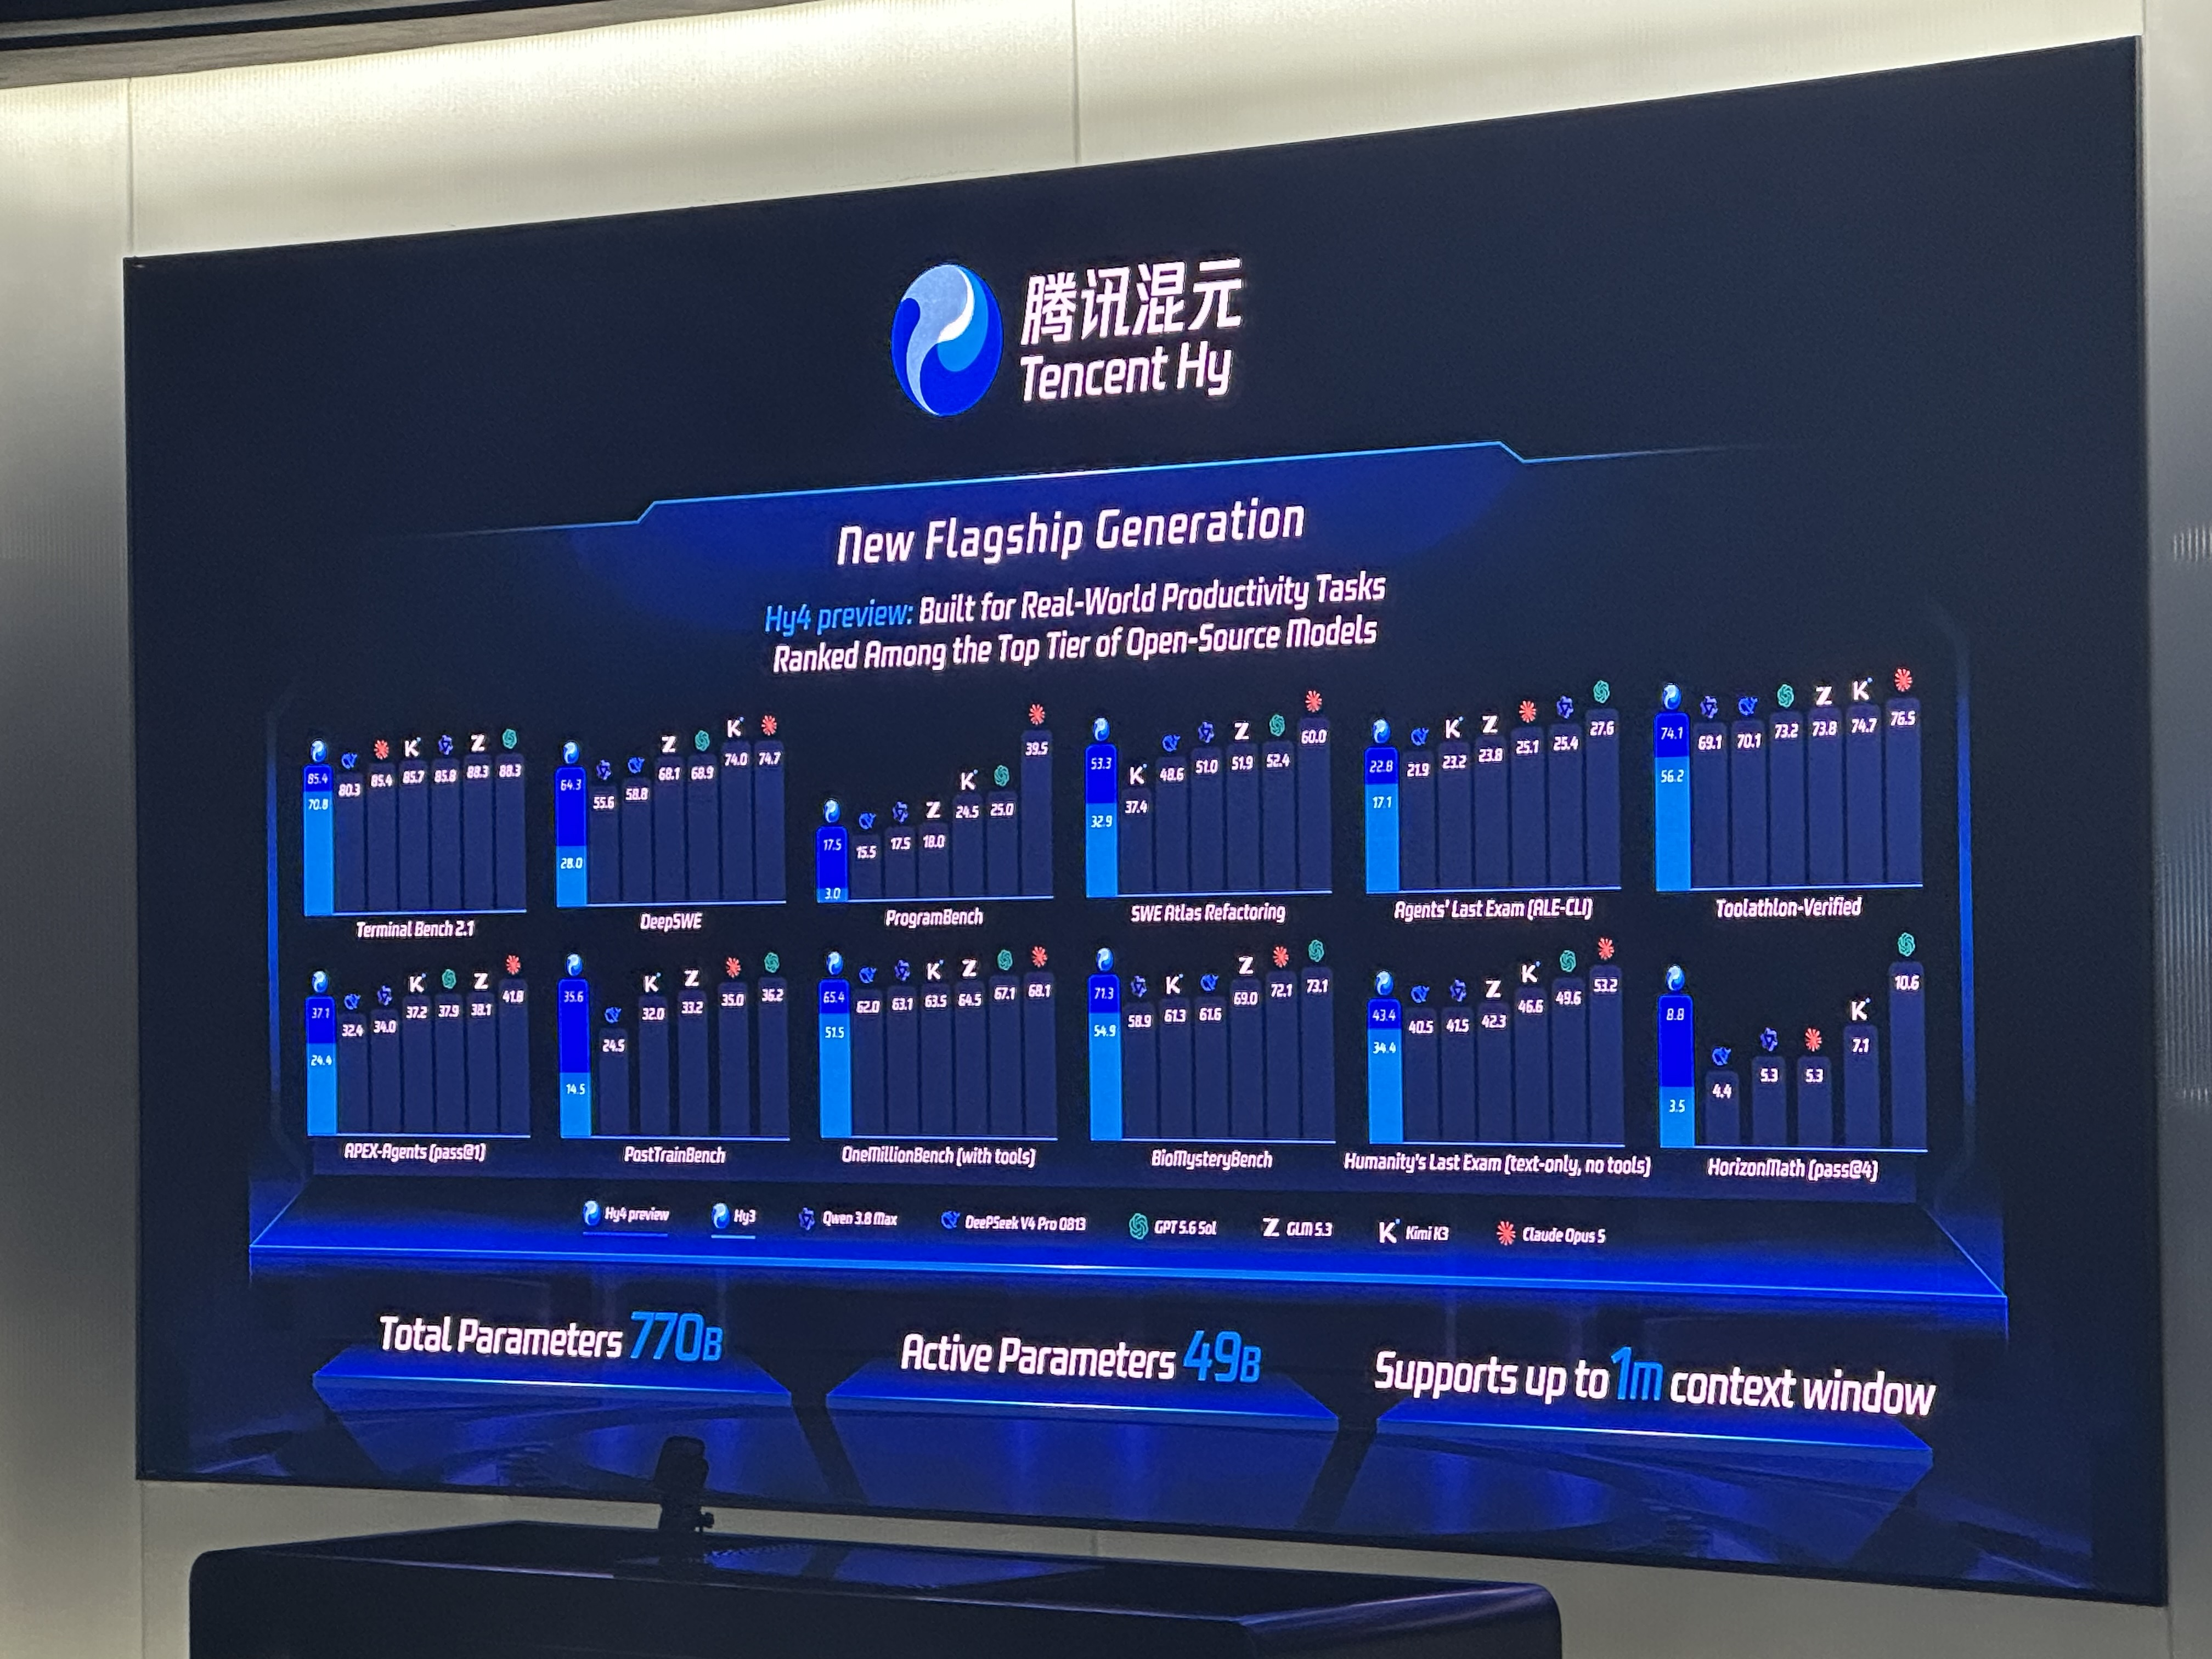
\includegraphics[width=\columnwidth]{figures/tencent_fieldtrip.jpg}
\caption{
Tencent Shanghai Office, September 4, 2026.
Photograph by Gihun Lee.
The displayed AI-model benchmark dashboard compares multiple models across
standardized evaluation tasks and model specifications. This observation
motivated the distinction between standardized model capability and
provider-specific consumer usage measures in the SUU proposal.
}
\Description{
A benchmark dashboard at Tencent Shanghai Office displaying comparative
performance information for multiple AI models.
}
\label{fig:tencent-field}
\end{figure}

\vspace{0.5em}

At \textbf{Shanghai Science and Technology Museum},
I observed wearable robotic assistance technology presented through practical
human applications.

This reinforced the principle that a useful technical metric should also be
interpretable to non-specialists.

\vspace{0.5em}

\begin{figure}[H]
\centering
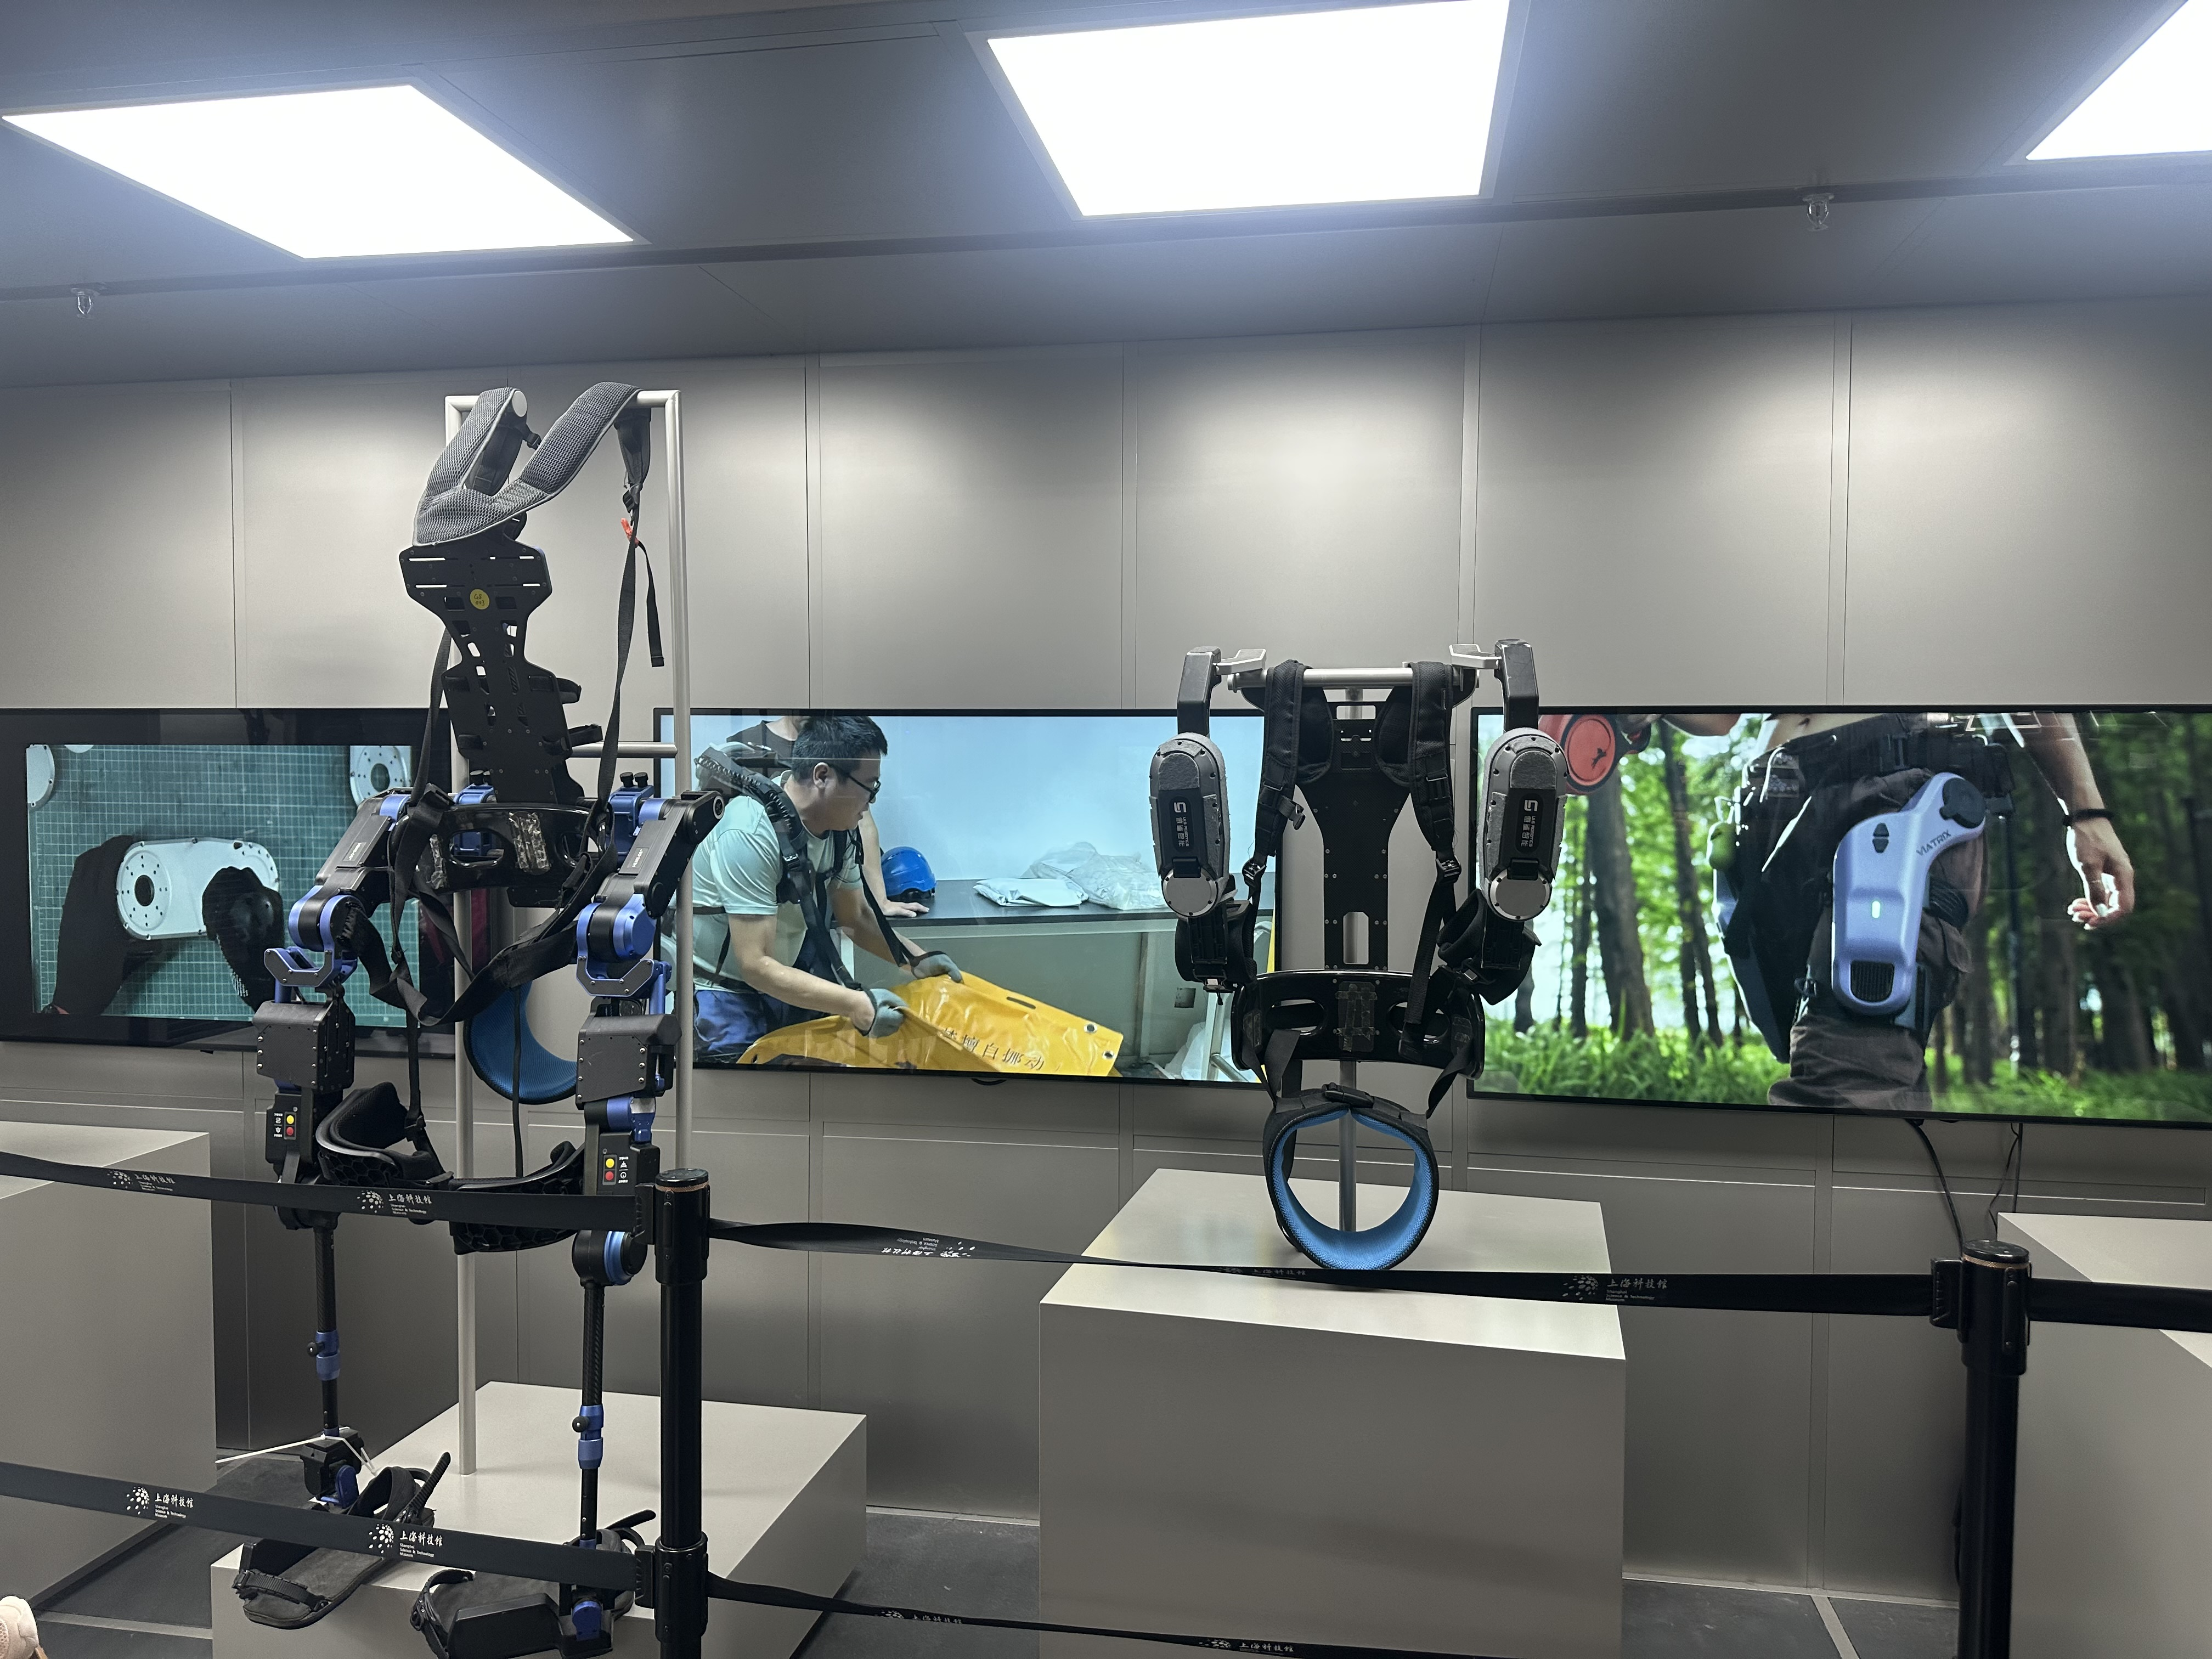
\includegraphics[width=\columnwidth]{figures/museum_fieldtrip.jpg}
\caption{
Shanghai Science and Technology Museum, September 4, 2026.
Photograph by Gihun Lee.
The exhibit demonstrates wearable robotic assistance for physical activity.
It motivated the design principle that technical AI-service measurements should
be translated into information that non-specialist users can understand and use.
}
\Description{
A wearable robotic assistance exhibit at Shanghai Science and Technology Museum
showing technology designed to support physical activity.
}
\label{fig:museum-field}
\end{figure}

\vspace{0.5em}

\subsection{Open-source inspirations}

\textbf{Industry---OpenTelemetry Generative AI Semantic Conventions.}
OpenTelemetry provides an open specification for recording telemetry from
GenAI systems, including common fields for usage and token-related activity.
I consulted the official OpenTelemetry project and the
\texttt{open-telemetry/semantic-conventions} repository,
licensed under Apache-2.0, accessed September 5, 2026.
Its main capability for this project is that it provides a common,
machine-readable vocabulary for recording GenAI activity.
Its limitation is that standardized recording does not establish an exchange
ratio between one provider's token or usage unit and another provider's unit.
This changed my proposal by suggesting that SUU should not replace existing
measurement infrastructure; instead, a vendor-neutral normalized usage unit
could be reported on top of shared telemetry conventions.

\begin{quote}
Official page:
\url{https://opentelemetry.io/}

Repository:
\url{https://github.com/open-telemetry/semantic-conventions}
\end{quote}

\textbf{Public sector---CKAN.}
CKAN is an open-source data-management platform used to publish, organize,
search, and provide API access to public datasets.
I consulted the official CKAN project and its source repository,
licensed under AGPLv3+, accessed September 5, 2026.
Its capability is to make public data machine-readable and accessible through
a common publication infrastructure.
Its limitation is that standardizing how data are published does not guarantee
that the underlying measurements are substantively comparable.
This changed my proposal by suggesting that SUU should eventually include not
only a mathematical definition but also a machine-readable reporting format
that public agencies could publish, inspect, and audit.

\begin{quote}
Official page:
\url{https://ckan.org/}

Repository:
\url{https://github.com/ckan/ckan}
\end{quote}

Together, these tools separate two layers of the proposal:
OpenTelemetry motivates standardized recording of AI-service activity,
while CKAN motivates transparent publication and auditability.
SUU addresses the remaining measurement problem by defining how heterogeneous
AI-service quantities could be normalized before they are reported or shared.

\vspace{0.5em}

The earlier reflection connected this work to SDG 16.6 through transparent
public procurement.
The PS1 Hugging Face artifact instead focuses directly on the required
SDG 4 educational contribution.


% ============================================================
% APPENDIX D
% ============================================================

\section{Review response and revision record}

\textbf{Version 1 status.}

The first reviewable proposal is submitted on September 13, 2026.
Peer reviews,
the author response,
reviewer follow-up,
and version 2 changes are pending.


% ============================================================
% APPENDIX E
% ============================================================

\clearpage
\onecolumn

\section{Structured abstract and cumulative proposal map}
\label{app:abstract}

\begin{table}[H]

\caption{
Appendix E structured abstract and cumulative proposal map.
}

\label{tab:abstract-map}

\renewcommand{\arraystretch}{1.18}

\begin{tabularx}{
\textwidth
}{
@{}
p{0.27\textwidth}
Y
@{}
}

\toprule

\textbf{Proposal element}
&
\textbf{Current statement / change}
\\

\midrule

Background
&
AI subscription services expose heterogeneous models and agents through
provider-specific messages,
tokens,
time windows,
weekly pools,
and feature-dependent restrictions.
Standardized model benchmarks exist,
but an equivalent consumer-facing measure of usable service quantity does not.
\\

Motivation and application
&
Consumers must jointly compare price,
capability,
and incompatibly defined usage limits.
The project develops a vendor-neutral usage measure while preserving
workload-specific differences so users can make more transparent comparisons.
\\

Three connected questions
&
Economics asks how standardized quality-aware information changes perceived
value;
computer science asks how heterogeneous limits and capabilities can be
normalized;
behavioral science asks whether standardization improves understanding or
induces anchoring.
The integrated question is whether a technically comparable unit can also be
economically meaningful and behaviorally useful.
\\

Method and model assumptions
&
The full framework defines
$\mathrm{SUU}_{p,j}=C_{p,j}B_{p,j}$.
The current PS1 computation implements the benchmark-quality component
$B_{p,j}$ using Artificial Analysis v4.3.
A normalized composite benchmark score serves as the baseline,
while the proposed modification reports separate Reasoning,
Coding, and Agentic benchmark components and their equal-weight Overall score.
The Colab performs one-at-a-time
$\pm10\%/\pm20\%$
sensitivity analysis on the raw benchmark inputs.
Provider-specific usage capacity $C_{p,j}$ remains planned future measurement.
\\

Results or expected results
&
The benchmark-normalization notebook produced Overall scores of 95.55 for
ChatGPT Plus, 95.06 for Claude Pro, 72.48 for Google AI Pro, and 75.28 for
SuperGrok. Workload-level results differed substantially; for example,
SuperGrok scored 94.66 on Agentic but 68.95 on Reasoning and 62.24 on Coding.
These are actual computational outputs from the frozen benchmark snapshot.
Final subscription-level SUU remains planned because provider-specific usage
capacity has not yet been measured.
\\

Intellectual merits
&
The proposal extends standardized AI comparison from capability alone toward
usable service quantity while avoiding a single opaque scalar measure.
Workload-specific SUUs preserve heterogeneity,
economic reasoning constrains interpretation,
and behavioral evaluation tests whether standardization helps rather than
merely simplifies.
\\

Practical impacts
&
SUU could make AI subscription comparison clearer for consumers and later
support procurement and reporting.
The Hugging Face artifact supports SDG 4 by teaching how usage limits,
quality,
and workload jointly determine usable service.
Learning effects remain to be tested.
\\

Feedback received and revision made
&
The project changed from an earlier film-industry trend question after the September 4 Tencent observation highlighted a gap between standardized AI
benchmarks and fragmented usage measures.
SUU was later revised from one scalar output to
Overall, Reasoning, Coding, and Agentic views to reduce false comparability.

\\

\bottomrule

\end{tabularx}

\end{table}


\end{document}